\documentclass[a4paper, 11pt]{article}
\usepackage{comment} % enables the use of multi-line comments (\ifx \fi) 
\usepackage{fullpage} % changes the margin
\usepackage[a4paper, total={7in, 10in}]{geometry}
\usepackage{amsmath,mathtools}
\usepackage{amssymb,amsthm}  % assumes amsmath package installed
\usepackage{float}
\usepackage{graphicx}
\graphicspath{{./images/}}
\usepackage{xcolor}
\usepackage{mdframed}
\usepackage[shortlabels]{enumitem}
\usepackage{indentfirst,multicol}
\usepackage{hyperref}
\hypersetup{
	colorlinks=true,
	linkcolor=blue,
	filecolor=magenta,      
	urlcolor=blue!70!red,
	pdftitle={Assignment}, %%%%%%%%%%%%%%%%   WRITE ASSIGNMENT PDF NAME  %%%%%%%%%%%%%%%%%%%%
}
\usepackage[most,many,breakable]{tcolorbox}



\definecolor{mytheorembg}{HTML}{F2F2F9}
\definecolor{mytheoremfr}{HTML}{00007B}


\tcbuselibrary{theorems,skins,hooks}
\newtcbtheorem{problem}{Problem}
{%
	enhanced,
	breakable,
	colback = mytheorembg,
	frame hidden,
	boxrule = 0sp,
	borderline west = {2pt}{0pt}{mytheoremfr},
	sharp corners,
	detach title,
	before upper = \tcbtitle\par\smallskip,
	coltitle = mytheoremfr,
	fonttitle = \bfseries\sffamily,
	description font = \mdseries,
	separator sign none,
	segmentation style={solid, mytheoremfr},
}
{p}

% To give references for any problem use like this
% suppose the problem number is p3 then 2 options either 
% \hyperref[p:p3]{<text you want to use to hyperlink> \ref{p:p3}}
%                  or directly 
%                   \ref{p:p3}


%---------------------------------------
% BlackBoard Math Fonts :-
%---------------------------------------

%Captital Letters
\newcommand{\bbA}{\mathbb{A}}	\newcommand{\bbB}{\mathbb{B}}
\newcommand{\bbC}{\mathbb{C}}	\newcommand{\bbD}{\mathbb{D}}
\newcommand{\bbE}{\mathbb{E}}	\newcommand{\bbF}{\mathbb{F}}
\newcommand{\bbG}{\mathbb{G}}	\newcommand{\bbH}{\mathbb{H}}
\newcommand{\bbI}{\mathbb{I}}	\newcommand{\bbJ}{\mathbb{J}}
\newcommand{\bbK}{\mathbb{K}}	\newcommand{\bbL}{\mathbb{L}}
\newcommand{\bbM}{\mathbb{M}}	\newcommand{\bbN}{\mathbb{N}}
\newcommand{\bbO}{\mathbb{O}}	\newcommand{\bbP}{\mathbb{P}}
\newcommand{\bbQ}{\mathbb{Q}}	\newcommand{\bbR}{\mathbb{R}}
\newcommand{\bbS}{\mathbb{S}}	\newcommand{\bbT}{\mathbb{T}}
\newcommand{\bbU}{\mathbb{U}}	\newcommand{\bbV}{\mathbb{V}}
\newcommand{\bbW}{\mathbb{W}}	\newcommand{\bbX}{\mathbb{X}}
\newcommand{\bbY}{\mathbb{Y}}	\newcommand{\bbZ}{\mathbb{Z}}

%---------------------------------------
% MathCal Fonts :-
%---------------------------------------

%Captital Letters
\newcommand{\mcA}{\mathcal{A}}	\newcommand{\mcB}{\mathcal{B}}
\newcommand{\mcC}{\mathcal{C}}	\newcommand{\mcD}{\mathcal{D}}
\newcommand{\mcE}{\mathcal{E}}	\newcommand{\mcF}{\mathcal{F}}
\newcommand{\mcG}{\mathcal{G}}	\newcommand{\mcH}{\mathcal{H}}
\newcommand{\mcI}{\mathcal{I}}	\newcommand{\mcJ}{\mathcal{J}}
\newcommand{\mcK}{\mathcal{K}}	\newcommand{\mcL}{\mathcal{L}}
\newcommand{\mcM}{\mathcal{M}}	\newcommand{\mcN}{\mathcal{N}}
\newcommand{\mcO}{\mathcal{O}}	\newcommand{\mcP}{\mathcal{P}}
\newcommand{\mcQ}{\mathcal{Q}}	\newcommand{\mcR}{\mathcal{R}}
\newcommand{\mcS}{\mathcal{S}}	\newcommand{\mcT}{\mathcal{T}}
\newcommand{\mcU}{\mathcal{U}}	\newcommand{\mcV}{\mathcal{V}}
\newcommand{\mcW}{\mathcal{W}}	\newcommand{\mcX}{\mathcal{X}}
\newcommand{\mcY}{\mathcal{Y}}	\newcommand{\mcZ}{\mathcal{Z}}



%---------------------------------------
% Bold Math Fonts :-
%---------------------------------------

%Captital Letters
\newcommand{\bmA}{\boldsymbol{A}}	\newcommand{\bmB}{\boldsymbol{B}}
\newcommand{\bmC}{\boldsymbol{C}}	\newcommand{\bmD}{\boldsymbol{D}}
\newcommand{\bmE}{\boldsymbol{E}}	\newcommand{\bmF}{\boldsymbol{F}}
\newcommand{\bmG}{\boldsymbol{G}}	\newcommand{\bmH}{\boldsymbol{H}}
\newcommand{\bmI}{\boldsymbol{I}}	\newcommand{\bmJ}{\boldsymbol{J}}
\newcommand{\bmK}{\boldsymbol{K}}	\newcommand{\bmL}{\boldsymbol{L}}
\newcommand{\bmM}{\boldsymbol{M}}	\newcommand{\bmN}{\boldsymbol{N}}
\newcommand{\bmO}{\boldsymbol{O}}	\newcommand{\bmP}{\boldsymbol{P}}
\newcommand{\bmQ}{\boldsymbol{Q}}	\newcommand{\bmR}{\boldsymbol{R}}
\newcommand{\bmS}{\boldsymbol{S}}	\newcommand{\bmT}{\boldsymbol{T}}
\newcommand{\bmU}{\boldsymbol{U}}	\newcommand{\bmV}{\boldsymbol{V}}
\newcommand{\bmW}{\boldsymbol{W}}	\newcommand{\bmX}{\boldsymbol{X}}
\newcommand{\bmY}{\boldsymbol{Y}}	\newcommand{\bmZ}{\boldsymbol{Z}}
%Small Letters
\newcommand{\bma}{\boldsymbol{a}}	\newcommand{\bmb}{\boldsymbol{b}}
\newcommand{\bmc}{\boldsymbol{c}}	\newcommand{\bmd}{\boldsymbol{d}}
\newcommand{\bme}{\boldsymbol{e}}	\newcommand{\bmf}{\boldsymbol{f}}
\newcommand{\bmg}{\boldsymbol{g}}	\newcommand{\bmh}{\boldsymbol{h}}
\newcommand{\bmi}{\boldsymbol{i}}	\newcommand{\bmj}{\boldsymbol{j}}
\newcommand{\bmk}{\boldsymbol{k}}	\newcommand{\bml}{\boldsymbol{l}}
\newcommand{\bmm}{\boldsymbol{m}}	\newcommand{\bmn}{\boldsymbol{n}}
\newcommand{\bmo}{\boldsymbol{o}}	\newcommand{\bmp}{\boldsymbol{p}}
\newcommand{\bmq}{\boldsymbol{q}}	\newcommand{\bmr}{\boldsymbol{r}}
\newcommand{\bms}{\boldsymbol{s}}	\newcommand{\bmt}{\boldsymbol{t}}
\newcommand{\bmu}{\boldsymbol{u}}	\newcommand{\bmv}{\boldsymbol{v}}
\newcommand{\bmw}{\boldsymbol{w}}	\newcommand{\bmx}{\boldsymbol{x}}
\newcommand{\bmy}{\boldsymbol{y}}	\newcommand{\bmz}{\boldsymbol{z}}

%---------------------------------------
% Scr Math Fonts :-
%---------------------------------------

\newcommand{\sA}{{\mathscr{A}}}   \newcommand{\sB}{{\mathscr{B}}}
\newcommand{\sC}{{\mathscr{C}}}   \newcommand{\sD}{{\mathscr{D}}}
\newcommand{\sE}{{\mathscr{E}}}   \newcommand{\sF}{{\mathscr{F}}}
\newcommand{\sG}{{\mathscr{G}}}   \newcommand{\sH}{{\mathscr{H}}}
\newcommand{\sI}{{\mathscr{I}}}   \newcommand{\sJ}{{\mathscr{J}}}
\newcommand{\sK}{{\mathscr{K}}}   \newcommand{\sL}{{\mathscr{L}}}
\newcommand{\sM}{{\mathscr{M}}}   \newcommand{\sN}{{\mathscr{N}}}
\newcommand{\sO}{{\mathscr{O}}}   \newcommand{\sP}{{\mathscr{P}}}
\newcommand{\sQ}{{\mathscr{Q}}}   \newcommand{\sR}{{\mathscr{R}}}
\newcommand{\sS}{{\mathscr{S}}}   \newcommand{\sT}{{\mathscr{T}}}
\newcommand{\sU}{{\mathscr{U}}}   \newcommand{\sV}{{\mathscr{V}}}
\newcommand{\sW}{{\mathscr{W}}}   \newcommand{\sX}{{\mathscr{X}}}
\newcommand{\sY}{{\mathscr{Y}}}   \newcommand{\sZ}{{\mathscr{Z}}}


%---------------------------------------
% Math Fraktur Font
%---------------------------------------

%Captital Letters
\newcommand{\mfA}{\mathfrak{A}}	\newcommand{\mfB}{\mathfrak{B}}
\newcommand{\mfC}{\mathfrak{C}}	\newcommand{\mfD}{\mathfrak{D}}
\newcommand{\mfE}{\mathfrak{E}}	\newcommand{\mfF}{\mathfrak{F}}
\newcommand{\mfG}{\mathfrak{G}}	\newcommand{\mfH}{\mathfrak{H}}
\newcommand{\mfI}{\mathfrak{I}}	\newcommand{\mfJ}{\mathfrak{J}}
\newcommand{\mfK}{\mathfrak{K}}	\newcommand{\mfL}{\mathfrak{L}}
\newcommand{\mfM}{\mathfrak{M}}	\newcommand{\mfN}{\mathfrak{N}}
\newcommand{\mfO}{\mathfrak{O}}	\newcommand{\mfP}{\mathfrak{P}}
\newcommand{\mfQ}{\mathfrak{Q}}	\newcommand{\mfR}{\mathfrak{R}}
\newcommand{\mfS}{\mathfrak{S}}	\newcommand{\mfT}{\mathfrak{T}}
\newcommand{\mfU}{\mathfrak{U}}	\newcommand{\mfV}{\mathfrak{V}}
\newcommand{\mfW}{\mathfrak{W}}	\newcommand{\mfX}{\mathfrak{X}}
\newcommand{\mfY}{\mathfrak{Y}}	\newcommand{\mfZ}{\mathfrak{Z}}
%Small Letters
\newcommand{\mfa}{\mathfrak{a}}	\newcommand{\mfb}{\mathfrak{b}}
\newcommand{\mfc}{\mathfrak{c}}	\newcommand{\mfd}{\mathfrak{d}}
\newcommand{\mfe}{\mathfrak{e}}	\newcommand{\mff}{\mathfrak{f}}
\newcommand{\mfg}{\mathfrak{g}}	\newcommand{\mfh}{\mathfrak{h}}
\newcommand{\mfi}{\mathfrak{i}}	\newcommand{\mfj}{\mathfrak{j}}
\newcommand{\mfk}{\mathfrak{k}}	\newcommand{\mfl}{\mathfrak{l}}
\newcommand{\mfm}{\mathfrak{m}}	\newcommand{\mfn}{\mathfrak{n}}
\newcommand{\mfo}{\mathfrak{o}}	\newcommand{\mfp}{\mathfrak{p}}
\newcommand{\mfq}{\mathfrak{q}}	\newcommand{\mfr}{\mathfrak{r}}
\newcommand{\mfs}{\mathfrak{s}}	\newcommand{\mft}{\mathfrak{t}}
\newcommand{\mfu}{\mathfrak{u}}	\newcommand{\mfv}{\mathfrak{v}}
\newcommand{\mfw}{\mathfrak{w}}	\newcommand{\mfx}{\mathfrak{x}}
\newcommand{\mfy}{\mathfrak{y}}	\newcommand{\mfz}{\mathfrak{z}}

%---------------------------------------
% Bar
%---------------------------------------

%Captital Letters
\newcommand{\barA}{\overline{A}}	\newcommand{\barB}{\overline{B}}
\newcommand{\barC}{\overline{C}}	\newcommand{\barD}{\overline{D}}
\newcommand{\barE}{\overline{E}}	\newcommand{\barF}{\overline{F}}
\newcommand{\barG}{\overline{G}}	\newcommand{\barH}{\overline{H}}
\newcommand{\barI}{\overline{I}}	\newcommand{\barJ}{\overline{J}}
\newcommand{\barK}{\overline{K}}	\newcommand{\barL}{\overline{L}}
\newcommand{\barM}{\overline{M}}	\newcommand{\barN}{\overline{N}}
\newcommand{\barO}{\overline{O}}	\newcommand{\barP}{\overline{P}}
\newcommand{\barQ}{\overline{Q}}	\newcommand{\barR}{\overline{R}}
\newcommand{\barS}{\overline{S}}	\newcommand{\barT}{\overline{T}}
\newcommand{\barU}{\overline{U}}	\newcommand{\barV}{\overline{V}}
\newcommand{\barW}{\overline{W}}	\newcommand{\barX}{\overline{X}}
\newcommand{\barY}{\overline{Y}}	\newcommand{\barZ}{\overline{Z}}
%Small Letters
\newcommand{\bara}{\overline{a}}	\newcommand{\barb}{\overline{b}}
\newcommand{\barc}{\overline{c}}	\newcommand{\bard}{\overline{d}}
\newcommand{\bare}{\overline{e}}	\newcommand{\barf}{\overline{f}}
\newcommand{\barg}{\overline{g}}	\newcommand{\barh}{\overline{h}}
\newcommand{\bari}{\overline{i}}	\newcommand{\barj}{\overline{j}}
\newcommand{\bark}{\overline{k}}	\newcommand{\barl}{\overline{l}}
\newcommand{\barm}{\overline{m}}	\newcommand{\barn}{\overline{n}}
\newcommand{\baro}{\overline{o}}	\newcommand{\barp}{\overline{p}}
\newcommand{\barq}{\overline{q}}	\newcommand{\barr}{\overline{r}}
\newcommand{\bars}{\overline{s}}	\newcommand{\bart}{\overline{t}}
\newcommand{\baru}{\overline{u}}	\newcommand{\barv}{\overline{v}}
\newcommand{\barw}{\overline{w}}	\newcommand{\barx}{\overline{x}}
\newcommand{\bary}{\overline{y}}	\newcommand{\barz}{\overline{z}}

%---------------------------------------
% Greek Letters:-
%---------------------------------------
\newcommand{\eps}{\epsilon}
\newcommand{\veps}{\varepsilon}
\newcommand{\lm}{\lambda}
\newcommand{\Lm}{\Lambda}
\newcommand{\gm}{\gamma}
\newcommand{\Gm}{\Gamma}
\newcommand{\vph}{\varphi}
\newcommand{\ph}{\phi}

\newcommand{\Qed}{\begin{flushright}\qed\end{flushright}}
\newcommand{\parinn}{\setlength{\parindent}{1cm}}
\newcommand{\parinf}{\setlength{\parindent}{0cm}}
\newcommand{\del}[2]{\frac{\partial #1}{\partial #2}}
\newcommand{\Del}[3]{\frac{\partial^{#1} #2}{\partial^{#1} #3}}
\newcommand{\deld}[2]{\dfrac{\partial #1}{\partial #2}}
\newcommand{\Deld}[3]{\dfrac{\partial^{#1} #2}{\partial^{#1} #3}}
\newcommand{\uin}{\mathbin{\rotatebox[origin=c]{90}{$\in$}}}
\newcommand{\usubset}{\mathbin{\rotatebox[origin=c]{90}{$\subset$}}}
\newcommand{\lt}{\left}
\newcommand{\rt}{\right}
\newcommand{\exs}{\exists}
\newcommand{\st}{\strut}
\newcommand{\dps}[1]{\displaystyle{#1}}
\newcommand{\la}{\langle}
\newcommand{\ra}{\rangle}
\newenvironment{solution}
{\textit{\textbf{Solution:}} 
}
{ 
	\hfill $\blacksquare$
	
	\vspace{1cm}
}
\newcommand{\sol}[1]{\begin{solution}#1\end{solution}}
\newcommand{\solve}[1]{\setlength{\parindent}{0cm}\textbf{\textit{Solution: }}\setlength{\parindent}{1cm}#1 \Qed}
\newcommand{\mat}[1]{\left[\begin{matrix}#1\end{matrix}\right]}
\newcommand\numberthis{\addtocounter{equation}{1}\tag{\theequation}}
\newcommand{\handout}[3]{
	\noindent
	\begin{center}
		\framebox{
			\vbox{
				\hbox to 6.5in { {\bf Complexity Theory I } \hfill Jan -- May, 2023 }
				\vspace{4mm}
				\hbox to 6.5in { {\Large \hfill #1  \hfill} }
				\vspace{2mm}
				\hbox to 6.5in { {\em #2 \hfill #3} }
			}
		}
	\end{center}
	\vspace*{4mm}
}

\newcommand{\lecture}[3]{\handout{Lecture #1}{Lecturer: #2}{Scribe:	#3}}
	

\newcommand{\ov}[1]{\overline{#1}}
\newcommand{\thmref}[1]{\hyperref[#1]{Theorem \ref{#1}}}
\newcommand{\Res}{\operatorname{Res}}

\setlength{\parindent}{0pt}

%%%%%%%%%%%%%%%%%%%%%%%%%%%%%%%%%%%%%%%%%%%%%%%%%%%%%%%%%%%%%%%%%%%%%%%%%%%%%%%%%%%%%%%%%%%%%%%%%%%%%%%%%%%%%%%%%%%%%%%%%%%%%%%%%%%%%%%%

\begin{document}
	
	%%%%%%%%%%%%%%%%%%%%%%%%%%%%%%%%%%%%%%%%%%%%%%%%%%%%%%%%%%%%%%%%%%%%%%%%%%%%%%%%%%%%%%%%%%%%%%%%%%%%%%%%%%%%%%%%%%%%%%%%%%%%%%%%%%%%%%%%
	
	\textsf{\noindent \large\textbf{Soham Chatterjee} \hfill \textbf{Assignment - 5}\\
		Email: \href{sohamc@cmi.ac.in}{sohamc@cmi.ac.in} \hfill Roll: BMC202175\\
		\normalsize Course: Complex Analysis \hfill Date: May 1, 2023}
	
	%%%%%%%%%%%%%%%%%%%%%%%%%%%%%%%%%%%%%%%%%%%%%%%%%%%%%%%%%%%%%%%%%%%%%%%%%%%%%%%%%%%%%%%%%%%%%%%%%%%%%%%%%%%%%%%%%%%%%%%%%%%%%%%%%%%%%%%%
	% Problem 1
	%%%%%%%%%%%%%%%%%%%%%%%%%%%%%%%%%%%%%%%%%%%%%%%%%%%%%%%%%%%%%%%%%%%%%%%%%%%%%%%%%%%%%%%%%%%%%%%%%%%%%%%%%%%%%%%%%%%%%%%%%%%%%%%%%%%%%%%%
	
	\begin{problem}{%problem statement
			Ahlfors Page 154: Problem 1
		}{p1% problem reference text
		}
How many roots does the equation $z^7-2 z^5+6 z^3-z+1=0$ have in the disk $|z|<1$ ? Hint: Look for the biggest term when $|z|=1$ and apply Rouche's theorem.
	\end{problem}
	
	\solve{
		%Solution
		Take $g(z)=z^7-2z^5+6z^3-z+1$ and $f(z)=6z^3$. Then on $|z|=1$ $$|g(z)-f(z)|=|z^7-2z^5-z+1|\leq |z|^7+2|z|^5+|z|+1\leq 1+2+1+1=5<6=|f(z)|$$Hence by Rouche's Theorem $f(z)$ and $g(z)$ has same number of zeros inside $|z|<1$. Now $f$ has only three zero (one zero with order three). Hence $g(z)$ has three zeros inside $|z|<1$. 
}
	
	
	%%%%%%%%%%%%%%%%%%%%%%%%%%%%%%%%%%%%%%%%%%%%%%%%%%%%%%%%%%%%%%%%%%%%%%%%%
	% Problem 2
	%%%%%%%%%%%%%%%%%%%%%%%%%%%%%%%%%%%%%%%%%%%%%%%%%%%%%%%%%%%%%%%%%%%%%%%%%
	
	\begin{problem}{%problem statement
			Ahlfors Page 154: Problem 2
		}{p2% problem reference text
		}
		%Problem		
How many roots of the equation $z^4-6 z+3=0$ have their modulus between 1 and 2 ?
	\end{problem}                               
	
	\solve{
		%Solution
		Let $g(z)=z^4-6z+3$. In this case we find how many zeros $g$ has inside $|z|<1$ and $|z|<2$. then we subtract the number of zeros inside the smaller disk from the number of zeros inside the bigger disk. \parinn 
		
		Take $f(z)=-6z$. Then on $|z|=1$ we have $$|g(z)-f(z)|=|z^4+3|\leq |z|^4+1= 4<6=|f(z)| $$
		Hence by Rouche's theorem $f$ and $g$ has same number of zeros inside $|z|<1$. Now $f$ has only one zero in $|z|<1$. Hence $g$ has one zero in $|z|<1$. 
		
		Now take $f(z)=z^4$. Then $|z|=2$ we have $$|g(z)-f(z)|=\-6z+3|\leq 6|z|+3=6\times 2+3=15<16=|f(z)|$$Hence by Rouche's Theorem $f$ and $g$ has same number of zeros inside $|z|<2$. Now $f$ has only four zeros in $|z|<2$ (one zero with order four). Therefore $g$ has four zeros in $|z|<2$. 
		
		Hence $g$ has $4-1=3$ zeros in the region between $|z|<1$ and $|z|<2$. 
		
		
}
	
	
	%%%%%%%%%%%%%%%%%%%%%%%%%%%%%%%%%%%%%%%%%%%%%%%%%%%%%%%%%%%%%%%%%%%%%%%%%
	% Problem 3
	%%%%%%%%%%%%%%%%%%%%%%%%%%%%%%%%%%%%%%%%%%%%%%%%%%%%%%%%%%%%%%%%%%%%%%%%%
	
	\begin{problem}{%problem statement
			Ahlfors Page 161: Problem 3
		}{p3% problem reference text
		}
		%Problem
Evaluate the following integrals by the method of residues:
\begin{multicols}{2}
	\begin{enumerate}[label=(\alph*)]
		\item ${\int\limits_0^{\pi / 2} \dfrac{d x}{a+\sin ^2 x},|a|>1}$,
		\item ${\int\limits_0^{\infty} \dfrac{x^2 d x}{x^4+5 x^2+6}}$,
		\item ${\int\limits_{-\infty}^{\infty} \dfrac{x^2-x+2}{x^4+10 x^2+9} d x}$,
		\item ${\int\limits_0^{\infty} \dfrac{x^2 d x}{\left(x^2+a^2\right)^3}, a}$ real,
		\item ${\int\limits_0^{\infty} \dfrac{\cos x}{x^2+a^2} d x}, a$  real,
		\item ${\int\limits_0^{\infty} \dfrac{x \sin x}{x^2+a^2} d x, a}$ real,
		\item ${\int\limits_0^{\infty} \dfrac{x^{1 / 3}}{1+x^2} d x}$,
		\item ${\int\limits_0^{\infty}\left(1+x^2\right)^{-1} \log x d x}$,
		\item ${\int\limits_0^{\infty} \log \left(1+x^2\right) \dfrac{d x}{x^{1+\alpha}}(0<\alpha<2)}$. (Try integration by parts.)
	\end{enumerate}
\end{multicols}	\end{problem}
	\pagebreak
	
	\solve{
		%Solution
		\begin{enumerate}[label=(\alph*)]
			\item We know $\sin^2 x=\frac{1-\cos  2x}{2}$ Hence $$\int_0^{\frac{\pi}{2}}\frac{dx}{a+\sin^2 x}=\int_0^{\frac{\pi}{2}}\frac{dx}{a+\frac{1-\cos2x}{2}}=\int_0^{\frac{\pi}2}\frac{2dx}{2a+1-\cos 2x}=\int_0^{\pi}\frac{dt}{2a+1-\cos t}\ [\text{Substituting $t=2x$}]$$Now take $-2a-1=b$. Threrefore $|b|>1$. Hence we need to evaluate $\dps{\int_{0}^{\pi}\frac{dx}{b-\cos x}}$
			
			\subsubsection*{Case 1: $b>1$}
			Then this is like Ahlfors Case 1 Example. Then $$\int_0^{\pi}\frac{dx}{b-\cos x}=\frac{\pi}{\sqrt{b^2-1}}=\frac{\pi}{\sqrt{(2a+1)^2-1}}=\frac{\pi}{2\sqrt{a}\sqrt{a+1}}$$
			
			\subsection*{Case 2: $b<-1$}
			Now  $$\int_0^{\pi}\frac{dx}{b+\cos x}=-i\int_{|z|=1}\frac{dz}{z^2+2bz+1}$$Hence $z^2+2bz+1=(z-\alpha)(z-\beta)$ where $$\alpha =-b+\sqrt{b^2-1}\quad \beta=-b-\sqrt{b^2-1}$$Then just like Ahlfors Case 1 Example instead of taking the root $\alpha =-b+\sqrt{b^2-1}$ we will choose the root $\beta =-b-\sqrt{b^2-1}$, cause $|\alpha|>1$ and $|\beta|<1$. Therefore residue at $\beta$ is $\frac1{\beta-\alpha}=-\frac1{2\sqrt{b^2-1}}$. Then we get $$\int_0^{\pi} \frac{dx}{b+\cos x}=-\frac{\pi}{\sqrt{b^-1}}=-\frac{\pi}{2\sqrt{a}\sqrt{a+1}}$$Therefore $$\int_0^{\frac{\pi}{2}}\frac{dx}{a+\sin^2 x}=\begin{cases}
				\dfrac{\pi}{2\sqrt{a}\sqrt{a+1}}& \text{when $a>1$}\\
				-\dfrac{\pi}{2\sqrt{a}\sqrt{a+1}}& \text{when $a<-1$}
			\end{cases}$$\qed
		
		\item $$\int_0^{\infty} \frac{x^2dx}{x^4+5x^2+6}=\frac12\int_{-\infty}^{\infty} \frac{x^2dx}{x^4+5x^2+6}$$Now this is like Ahlfors Case 2. Using that we get $$\int _{-\infty}^{\infty}\frac{x^2dx}{x^4+5x^2+6}=2\pi i \sum_{y>0}\operatorname{Res}\frac{z^2}{z^4+5z^2+6}$$Now $$z^4+5z^2+6=(z^2+3)(z^2+2)=(z+\sqrt{2}i)(z-\sqrt{2}i)(z+\sqrt{3}i)(z-\sqrt{3}i)$$Now \begin{align*}
			\Res_{z=\sqrt{3}i} \frac{z^2}{z^4+5z^2+6} & =\lim\limits_{z\to \sqrt{3}i}\frac{z^2(z-\sqrt{3}i)}{z^4+5z^2+6}=\frac{-3}{2\sqrt{3}i(-3+2)}=\frac{\sqrt{3}}{2i} \\
			\Res_{z=\sqrt{2}i} \frac{z^2}{z^4+5z^2+6} & =\lim\limits_{\to \sqrt{2}i}\frac{z^2(z-\sqrt{2}i)}{z^4+5z^2+6}=\frac{-2}{2\sqrt{2}i(-2+3)}=-\frac{\sqrt{2}}{2i}
		\end{align*}Therefore \begin{align*}
		2\pi i \sum_{y>0}\operatorname{Res}\frac{z^2}{z^4+5z^2+6}& =2\pi i\lt( 	\Res_{z=\sqrt{3}i} \frac{z^2}{z^4+5z^2+6}+	\Res_{z=\sqrt{2}i} \frac{z^2}{z^4+5z^2+6}\rt)\\
		&  = 2\pi i \lt(\frac{\sqrt{3}}{2i} -\frac{\sqrt{2}}{2i}\rt)=\pi(\sqrt{3}-\sqrt{2})
	\end{align*}Hence $$\int_0^{\infty} \frac{x^2dx}{x^4+5x^2+6}=\frac{\pi}{2}(\sqrt{3}-\sqrt{2})$$\qed

\item Now this is like Ahlfors Case 2. Using that we get $$\int_{-\infty}^{\infty}\frac{x^2-x+2}{x^4+10x^2+9}=2\pi i \sum_{y>0}\Res\frac{z^2-z+2}{z^4+10z^2+9}$$Now $$z^4+10z^2+9=(z^2 + 9)(z^2 + 1) = (z + 3i)(z - 3i)(z + i)(z - i)$$Now \begin{align*}
	\Res_{z=3i}\frac{z^2-z+2}{z^4+10z^2+9} & =\lim\limits_{z\to 3i}\frac{(z^2-z+2)(z-3i)}{z^4+10z^2+9}=\frac{-9 - 3i + 2}{6i(-9 + 1)}=\frac{7 + 3i}{48i} \\
	\Res_{z=i} \frac{z^2-z+2}{z^4+10z^2+9} & =\lim\limits_{z\to i} \frac{(z^2-z+2)(z- i)}{z^4+10z^2+9}=\frac{-1 - i +  2}{(-1 + 9)2i}=\frac{1-i}{16i}=\frac{3 - 3i}{48i}
\end{align*}Therefore \begin{align*}
	2\pi i \sum_{y>0}\operatorname{Res}\frac{z^2}{z^4+5z^2+6}& =2\pi i\lt( 	\Res_{z=3i}\frac{z^2-z+2}{z^4+10z^2+9}+	\Res_{z=i} \frac{z^2-z+2}{z^4+10z^2+9}\rt)\\
	&  = 2\pi i \lt(\frac{7 + 3i}{48i}+\frac{3 - 3i}{48i}\rt)=\pi\frac{10}{24}=\frac{5\pi}{12}
\end{align*}Hence $$\int_{-\infty}^{\infty}\frac{x^2-x+2}{x^4+10x^2+9}=\frac{5\pi}{12}$$\qed

\item If $a=0$ then the integral is infinite. Hence lets assume $a\neq 0$. $$\int_0^{\infty} \frac{x^2dx}{(x^2+a^2)^3}=\frac12\int_{-\infty}^{\infty} \frac{x^2dx}{(x^2+a^2)^3}$$Now this is like Ahlfors Case 2. Using that we get $$\int _{-\infty}^{\infty}\frac{x^2dx}{(x^2+a^2)^3}=2\pi i \sum_{y>0}\operatorname{Res}\frac{z^2}{(z^2+a^2)^3}$$Now $$(z^2+a^2)^3=(z+ai)^3(z-ai)^3$$Now WLOG assume $a>0$. Now $$\frac{d^2}{dz^2}\frac{z^2(z-ai)^3}{(z^2+a^2)^3}=\frac{d}{dz}\lt[  \frac{2z}{(z+ai)^3}-\frac{3z^2}{(z+ai)^4}\rt]=\frac{d^2}{dz^2}\frac{z^2}{(z+ai)^3}=\frac{2}{(z+ai)^3}-\frac{12z^2}{(z+ai)^4}+\frac{12z^2}{(z+ai)^5}$$  \begin{align*}
	\Res_{z=ai} \frac{z^2}{(z^2+a^2)^3} & =\lim\limits_{z\to ai}\frac1{2!}\frac{d^2}{dz^2}\frac{z^2(z-ai)^3}{(z^2+a^2)^3}=\frac{1}{2} \lim _{z \rightarrow a i}\left(\frac{2}{(z+a i)^3}-\frac{12 z}{(z+a i)^4}+\frac{12 z^2}{(z+a i)^5}\right)=\frac{1}{16 a^3 i}\\
	\Res_{z=-ai} \frac{z^2}{(z^2+a^2)^3} & =\lim\limits_{z\to -ai}\frac1{2!}\frac{d^2}{dz^2}\frac{z^2(z+ai)^3}{(z^2+a^2)^3}=\frac{1}{2} \lim _{z \rightarrow -a i}\left(\frac{2}{(z-a i)^3}-\frac{12 z}{(z-a i)^4}+\frac{12 z^2}{(z-a i)^5}\right)=-\frac{1}{16 a^3 i}
\end{align*}Therefore \begin{align*}
2\pi i \sum_{y>0}\operatorname{Res}\frac{z^2}{(z^2+a^2)^3}=\begin{cases}
	2\pi i	\Res_{z=ai} \dfrac{z^2}{(z^2+a^2)^3}  = 2\pi i \dfrac{1}{16 a^3 i}=\dfrac{2\pi}{16a^3} & \text{when $a>0$}\\
	2\pi i	\Res_{z=-ai} \dfrac{z^2}{(z^2+a^2)^3}  = 2\pi i \dfrac{1}{16 (-a)^3 i}=\dfrac{2\pi}{16(-a)^3} & \text{when $a<0$}
\end{cases}
\end{align*}Hence $$\int_0^{\infty} \frac{x^2dx}{x^4+5x^2+6}= \frac{\pi}{16|a|^3}\quad \text{when }a\neq 0$$\qed


\item If $a=0$ then $$\int_0^{\infty}\frac{\cos x}{x^2}dx\geq -\int_0^{\infty}\frac{dx}{x^2}$$ which is divergent hence the integral is infinite. Hence lets assume $a\neq 0$. Since $\frac{\sin x}{x^2+a^2}$ is an odd function we have $\dps{\int\limits_{-\infty}^{\infty}\frac{\sin x}{x^2+a^2}dx=0}$. Hence we have $$\int_0^{\infty}\frac{\cos x}{x^2+a^2}dx=\frac12\int_{-\infty}^{\infty}\frac{\cos x}{x^2+a^2}dx=\frac12\lt[ \int_{-\infty}^{\infty}\frac{\cos x}{x^2+a^2}dx +i\int_{-\infty}^{\infty}\frac{\sin x}{x^2+a^2}\rt]=\frac12\int_{-\infty}^{\infty}\frac{e^{ix}dx}{x^2+a^2}$$ Now this is like Ahlfors Case 3 $$\int_{-\infty}^{\infty}\frac{e^{ix}dx}{x^2+a^2}=2\pi i\sum\limits_{y>0} \Res \frac{e^{iz}}{z^2+a^2}$$now $z^2+a^2=(z+ai)(a-ai)$. WLOG assume $a>0$ $$\Res_{z=ai}\frac{e^{iz}}{z^2+a^2}=\lim\limits_{z\to ai} \frac{e^{iz}(z-ai)}{z^2+a^2}=\frac{e^{-a}}{2ai}$$ Hence $$2\pi i\sum\limits_{y>0}\Res \frac{1}{z^2+a^2}=2\pi i\Res_{z=ai}\frac{e^{iz}}{z^2+a^2}=2\pi i \frac{e^{-a}}{2ai}=\frac{\pi e^{-a}}{a}$$Hence  $$\int_0^{\infty}\frac{\cos x}{x^2+a^2}dx=\frac{\pi e^{-a}}{2a}$$\qed

\item If $a=0$ then we have $ \dps{\int_0^{\infty}\frac{\sin x}{x}dx}=\frac{\pi}{2}]$ by Ahlfors Case 3 Example (Page 158)

Since $\frac{x\cos  x}{x^2+a^2}$ is an odd function we have $\dps{\int\limits_{-\infty}^{\infty}\frac{x\cos  x}{x^2+a^2}dx=0}$. Hence we have 
$$i\int_0^{\infty}\frac{x\sin x}{x^2+a^2}dx=i\frac12\int_{-\infty}^{\infty}\frac{x\sin x}{x^2+a^2}dx=\frac12\lt[ \int_{-\infty}^{\infty}\frac{x\sin x}{x^2+a^2}dx +i\int_{-\infty}^{\infty}\frac{x\cos x}{x^2+a^2}\rt]=\frac12\int_{-\infty}^{\infty}\frac{xe^{ix}dx}{x^2+a^2}$$Now this is like Ahlfors Case 3
$$\int_{-\infty}^{\infty}\frac{xe^{ix}dx}{x^2+a^2}=2\pi i\sum\limits_{y>0} \Res \frac{ze^{iz}}{z^2+a^2}$$

now $z^2+a^2=(z+ai)(a-ai)$. WLOG assume $a>0$ $$\Res_{z=ai}\frac{ze^{iz}}{z^2+a^2}=\lim\limits_{z\to ai} \frac{ze^{iz}(z-ai)}{z^2+a^2}=\frac{aie^{-a}}{2ai}=\frac{e^{-a}}2$$ Hence $$2\pi i\sum\limits_{y>0}\Res \frac{1}{z^2+a^2}=2\pi i\Res_{z=ai}\frac{ze^{iz}}{z^2+a^2}=2\pi i \frac{e^{-a}}{2}=\pi e^{-a}i$$Hence  $$\int_0^{\infty}\frac{x\sin x}{x^2+a^2}dx=\Im \lt(\frac12\pi e^{-a}i\rt)=\frac{\pi e^{-a}}{2}$$\qed

\item Now this is like Ahlfors Case 4. Hence we  have $$\int_0^\infty\frac{x^{1/3}dx}{1+x^2}= \frac{2}{1-e^{2\pi i/3}} \sum \Res \frac{z^{\frac13}}{1+z^2}$$ Now $$1+z^2=(z+i)(z-i)$$ Hence \begin{align*}
	\Res_{z=i}&=\lim\limits_{z\to i}\frac{z^{\frac13}(z-i)}{1+z^2}=\frac{i^{\frac13}}{2i}=\frac{e^{\frac{i\pi}{6}}}2\\
	\Res_{z=-i}&=\lim\limits_{z\to -i}\frac{z^{\frac13}(z+i)}{1+z^2}=\frac{(-i)^{\frac13}}{-2i}=-\frac{e^{\frac{i\pi}{2}}}2
\end{align*}Hence \begin{align*}
\frac{2}{1-e^{2\pi i/3}} \sum \Res \frac{z^{\frac13}}{1+z^2} & = \frac{2}{1-e^{2\pi i/3}}\lt[ \frac{e^{\frac{i\pi}{6}}}2- \frac{e^{\frac{i\pi}{2}}}2\rt]\\
& = \frac1{(1-e^{\pi i/3})({1+e^{\pi i/3}})}e^{\frac{i\pi}6}\lt( 1-e^{\frac{i\pi}3} \rt)\\
& = \frac{\pi e^{\frac{i\pi}6}}{1+e^{\frac{i\pi}3}}=\frac{\pi}{ e^{-\frac{i\pi}6}+e^{\frac{i\pi}6}}=\frac{\pi}{2\cos \frac{\pi}6}=\frac{\pi}{\sqrt{3}}
\end{align*}
Hence $$\int_0^\infty\frac{x^{1/3}dx}{1+x^2}=\frac{\pi}{\sqrt{3}}$$\qed
\pagebreak

\item Let $\gm$ be the following curve for $0<r<R$

\begin{figure}[h]
	\centering
	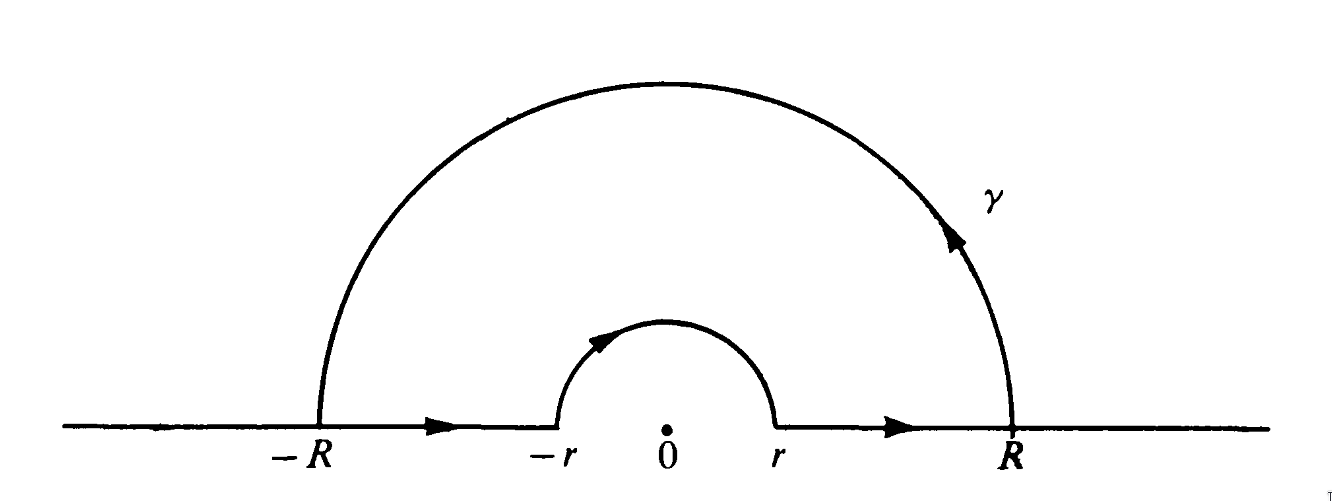
\includegraphics[width=10cm]{logxint.png}
\end{figure}


\begin{align*}
	\int_{\gm}\frac{\log z}{1+z^2}dz= \int_r^R \frac{\log x}{1+x^2} d x+i R \int_0^\pi \frac{\log R+i \theta}{1+R^2 e^{2 i \theta}} e^{i \theta} d \theta +\int_{-R}^{-r} \frac{\log |x|+\pi i}{1+x^2} d x+i r \int_\pi^0 \frac{[\log r+i \theta]}{1+r^2 e^{2 i \theta}} e^{i \theta} d \theta
\end{align*}Now

$$\int_{{r}}^R \frac{\log x}{1+x^2} d x+\int_{-R}^{-r} \frac{\log |x|+\pi i}{1+x^2} d x=2 \int_{{r}}^R \frac{\log x}{1+x^2} d x+\pi i \int_{{r}}^R \frac{d x}{1+x^2}$$Now as $r\to 0$ and $R\to \infty$ we have $$\int_{{r}}^R \frac{d x}{1+x^2}=\frac{\pi}{2}$$ Now

$$
	\left|R \int_0^\pi \frac{[\log R+i \theta]}{1+R^2 e^{i \theta}} e^{i \theta} d \theta\right|  \leq \frac{R|\log R|}{\left|1-R^2\right|} \int_0^\pi d \theta+\frac{R}{\left|1-R^2\right|} \int_0^\pi \theta d \theta  =\frac{\pi R|\log R|}{\left|1-R^2\right|}+\frac{R \pi^2}{2\left|1-R^2\right|} 
$$
Hence as $R\to \infty$ we have $\frac{\pi R|\log R|}{\left|1-R^2\right|}+\frac{R \pi^2}{2\left|1-R^2\right|} \to 0$. Similarly $$	\left|r \int_0^\pi \frac{[\log r+i \theta]}{1+r^2 e^{i \theta}} e^{i \theta} d \theta\right|  \leq \frac{r|\log r|}{\left|1-r^2\right|} \int_0^\pi d \theta+\frac{r}{\left|1-r^2\right|} \int_0^\pi \theta d \theta  =\frac{\pi r|\log r|}{\left|1-r^2\right|}+\frac{r \pi^2}{2\left|1-r^2\right|} $$Hence as $r\to 0$ we have $\frac{\pi r|\log r|}{\left|1-r^2\right|}+\frac{r \pi^2}{2\left|1-r^2\right|}\to 0$. Now by Residue Theorem we have $$	\int_{\gm}\frac{\log z}{1+z^2}dz=\sum_{y>0} \Res \frac{\log z}{1+z^2}$$ Now $1+z^2=(z+i)(z-i)$. Therefore $$\Res_{z=i}\frac{\log z}{1+z^2}=\lim\limits_{z\to i}\frac{(z-i)\log z}{1+z^2}=\frac{\log i}{2i}=\frac{\frac{i\pi}{2}}{2i}=\frac{\pi}{4}$$Hence $$\int_{\gm}\frac{\log z}{1+z^2}dz=2\pi i\frac{\pi}{4}=\frac{\pi^2i}{2}=2\int_0^{\infty}\frac{\log x}{1+x^2}dx+\pi i\frac{\pi}2\implies \int_0^{\infty}\frac{\log x}{1+x^2}dx=0$$


\item $$	\int_0^{\infty} \frac{\log \left(1+x^2\right)}{x^{1+\alpha}} d x =-\left.\frac{\log \left(1+x^2\right)}{\alpha x^\alpha}\right|_0 ^{\infty}+\frac{1}{\alpha} \int_0^{\infty} \frac{d / d x \log \left(1+x^2\right)}{x^\alpha} d x  =\frac{2}{\alpha} \int_0^{\infty} \frac{x}{x^\alpha\left(1+x^2\right)} d x$$Now there are three cases
\subsubsection*{Case 1: $\alpha=1$}

Then $$\frac{2}{\alpha} \int_0^{\infty} \frac{x}{x^\alpha\left(1+x^2\right)} d x= 2\int_0^{\infty} \frac{x}{x\left(1+x^2\right)} d x=2\int_0^{\infty} \frac{1}{\left(1+x^2\right)} d x=2\frac{\pi}{2}=\pi$$

\subsubsection*{Case 2: $0<\alpha<1$}
Then take $a=1-\alpha$. Then $0<a<1$. Hence $$\int_0^{\infty} \frac{x}{x^\alpha\left(1+x^2\right)} d x= \int_0^{\infty} \frac{x^{1-\alpha}}{1+x^2} d x= \int_0^{\infty} \frac{x^a}{1+x^2} d x$$This is like Ahlfors Case 4.  Now $1+z^2=(z+i)(z-i)$. Hence $$\Res_{z=i}\frac{z^a}{1+z^2}=\lim\limits_{z\to i}\frac{z^a(z-i)}{1+z^2}=\frac{i^a}{2i}=\frac{e^{\frac{ia\pi}{2}}}{2i}$$
$$\Res_{z=-i}\frac{z^a}{1+z^2}=\lim\limits_{z\to -i}\frac{z^a(z+i)}{1+z^2}=\frac{(-i)^a}{-2i}=-\frac{e^{\frac{i3a\pi}{2}}}{2i}$$ Hence \begin{align*}
	\int_0^{\infty} \frac{x}{x^\alpha\left(1+x^2\right)} d x & =\frac{2\pi i}{1-e^{2\pi i a}}\lt[ \frac{e^{\frac{ia\pi}{2}}}{2i}-\frac{e^{\frac{i3a\pi}{2}}}{2i} \rt]                         \\
	                                                         & = \frac{\pi e^{\frac{ia\pi}{2}}}{(1-e^{\pi i a})(1+e^{\pi i a})}\lt(1-e^{\pi i a}  \rt)                                        \\
	                                                         & = \frac{\pi e^{\frac{ia\pi}{2}}}{1+e^{\pi i a}}                                                                                \\
	                                                         & = \frac{\pi}{e^{-\frac{ia\pi}{2}}+e^{\frac{ia\pi}{2}}}=\frac{\pi}{2\cos \frac{a\pi}{2}}=\frac{\pi}{2\sin \frac{\alpha \pi}{2}}
\end{align*}
Hence $$	\int_0^{\infty} \frac{\log \left(1+x^2\right)}{x^{1+\alpha}} d x=\frac{2}{\alpha} \, \frac{\pi}{2\sin \frac{\alpha \pi}{2}}=\frac{\pi}{\alpha\sin \frac{\alpha \pi}{2}}$$
\subsubsection*{Case 3: $1<\alpha<2$}
Then take $b=\alpha-1$. Then $0<b<1$. Hence $$\int_0^{\infty} \frac{x}{x^\alpha\left(1+x^2\right)} d x= \int_0^{\infty} \frac{1}{x^{\alpha-1}(1+x^2)} d x= \int_0^{\infty} \frac{1}{x^b(1+x^2)} d x$$Let $\gm$ be the following curve for $0<r<R$. 

\begin{figure}[h]
	\centering
	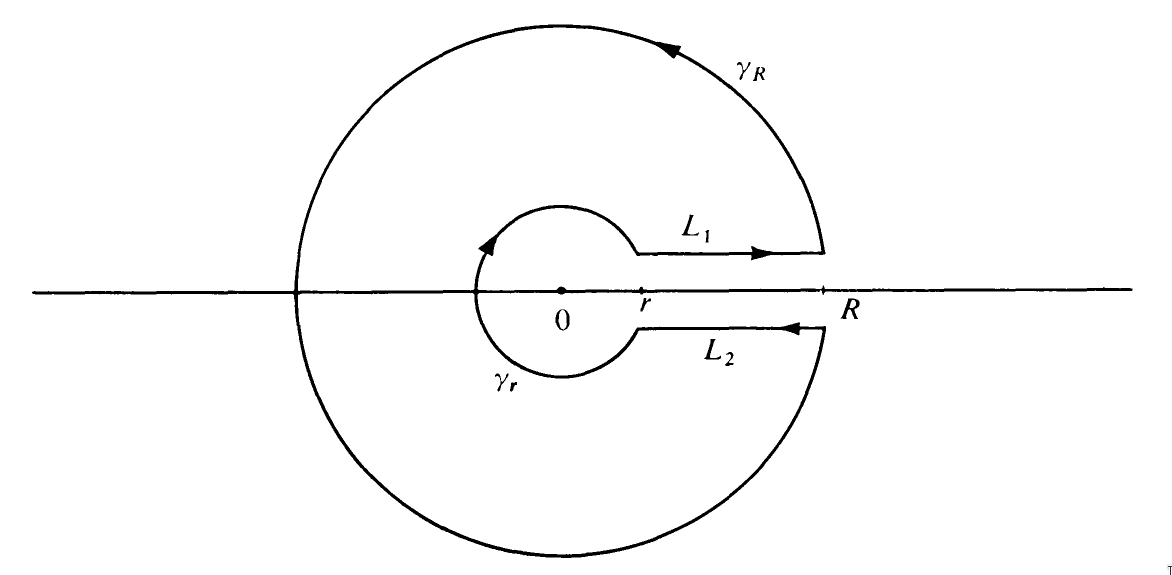
\includegraphics[width=10cm]{keyhole.png}
\end{figure}

Hence $$\left|\int_{\gamma_R} \frac{1}{z^b \left(1+z^2\right)} d z\right| \leq \frac{\pi R}{R^{\alpha-1}\left|R^2-1\right|}=\frac{\pi R^{2-\alpha}}{\left|R^2-1\right|}$$Since $1<\alpha<2$ we have $0<2-\alpha<1$. Hence as $R\to \infty$, $\frac{\pi R^{2-\alpha}}{\left|R^2-1\right|}\to 0$. Similarly $$\left|\int_{\gamma_r} \frac{1}{z^b \left(1+z^2\right)} d z\right| \leq \frac{\pi r}{r^{\alpha-1}\left|r^2-1\right|}=\frac{\pi r^{2-\alpha}}{\left|r^2-1\right|}$$Hence as $r\to 0$ we have $\frac{\pi r^{2-\alpha}}{\left|r^2-1\right|}\to 0$ Now $1+z^2=(z+i)(z-i)$. Hence 
$$\Res_{z= i}\frac{1}{z^b(1+z^2)}=\lim\limits_{z\to  i}\frac{z-i}{z^b(1+z^2)}=\frac{i^{-b}}{2i}=\frac{e^{-\frac{ib\pi}{2}}}{2i}$$
$$\Res_{z=-i}\frac{1}{z^b(1+z^2)}=\lim\limits_{z\to -i}\frac{z+i}{z^b(1+z^2)}=\frac{(-i)^{-b}}{-2i}=-\frac{e^{-\frac{i3b\pi}{2}}}{2i}$$Hence \begin{align*}
	\int_0^{\infty} \frac{1}{x^b(1+x^2)} d x & =\frac{2\pi i}{1-e^{-2\pi i b}}\lt[\frac{e^{-\frac{ib\pi}{2}}}{2i}-\frac{e^{-\frac{i3b\pi}{2}}}{2i} \rt]                       \\
	                                         & = \frac{\pi e^{-\frac{ib\pi}{2}}}{(1-e^{-\pi i b})(1+e^{-\pi i b})}\lt(1-e^{-\pi i b}  \rt)                                    \\
	                                         & = \frac{\pi e^{-\frac{ib\pi}{2}}}{1+e^{-\pi i b}}                                                                              \\
	                                         & = \frac{\pi}{e^{\frac{ib\pi}{2}}+e^{-\frac{ib\pi}{2}}}=\frac{\pi}{2\cos \frac{b\pi}{2}}=\frac{\pi}{2\sin \frac{\alpha \pi}{2}}
\end{align*}Hence $$	\int_0^{\infty} \frac{\log \left(1+x^2\right)}{x^{1+\alpha}} d x=\frac{2}{\alpha} \, \frac{\pi}{2\sin \frac{\alpha \pi}{2}}=\frac{\pi}{\alpha\sin \frac{\alpha \pi}{2}}$$

Therefore we get $\forall\ 0<\alpha <2$ we have $$	\int_0^{\infty} \frac{\log \left(1+x^2\right)}{x^{1+\alpha}} d x=\frac{2}{\alpha} \, \frac{\pi}{2\sin \frac{\alpha \pi}{2}}=\frac{\pi}{\alpha\sin \frac{\alpha \pi}{2}}$$

		\end{enumerate}	}
	



	
	%%%%%%%%%%%%%%%%%%%%%%%%%%%%%%%%%%%%%%%%%%%%%%%%%%%%%%%%%%%%%%%%%%%%%%%%%
	% Problem 4
	%%%%%%%%%%%%%%%%%%%%%%%%%%%%%%%%%%%%%%%%%%%%%%%%%%%%%%%%%%%%%%%%%%%%%%%%%

	
	\begin{problem}{%problem statement
			Ahlfors Page 186: Problem 2
		}{p4% problem reference text
		}
		%Problem		
Let $\Omega$ be a doubly connected region whose complement consists of the components $E_1, E_2$. Prove that every analytic function $f(z)$ in $\Omega$ can be written in the form $f_1(z)+f_2(z)$ where $f_1(z)$ is analytic outside of $E_1$ and $f_2(z)$ is analytic outside of $E_2$. (The precise proof requires a construction like the one in Chap. 4 , Sec. 4.5.)	\end{problem}
	
	\solve{
		%Solution
		Let $\Om$ be the given doubly connected region. At least one of the regions $E_1$ and $E_2$ is bounded. WLOG suppose $E_1$ is bounded. Hence boundary of $E_1$, $\partial E_1$ is compact. Hence $\partial E_2$ is closed and disjoint. Let distance between $\partial E_1$ and $\partial E_2$ is $d>0$
		
		Now we cover the entire plane with the grid of squares of length $\eps$. We will choose the $\eps>0$ later. Let $S$ be the set of squares which intersects $E_1$ Since $E_1$ is bounded $S$ is a finite set. Let $S'$ be the set of squares which are not in $S$ but intersects any square in $S$. Take the set $T=S\cup S'$. If we take $\eps$ sufficiently small then we can make $T\subset \Om$, take $\eps < \frac{\delta}{8}$
		
		Now we will define a cycle. $$\gm =\sum_{R\in S'}\partial R$$Now we cancel out the opposite directions of same sides. Now each side of $\gm$ have two cases\begin{enumerate}[label=(\arabic*)]
			\item An edge shared between a square in $S$ and an square in $S'$. 
			\item An outer edge of a square in $S'$.
		\end{enumerate}
Let $\gm_1$ be the part of $\gm$ which are of type $(1)$. And $\gm_2$ be the part of $\gm $ which are of type $(2)$. Hence they are disjoint and  $\gm_1$ is negatively oriented, $\gm_2$ is positively oriented.$$\gm_1+\gm_2=\gm$$Therefore $$\forall \ z\in E_1,\ n(\gm,z)=n(\gm_1,z)+n(\gm_2,z)=-1+1=0$$Similarly since $E_2$ is unbounded  we have $$\forall \ z\in E_2,\ n(\gm,a)=0$$since we can make $\eps$ small enough so that $E_2$ lies outside the region enclosed by $\gm_2$.  Hence $\gm\sim 0\pmod \Om$. 

Hence by Generalized Cauchy Theorem $$f_k(z)=\frac{1}{2\pi i}\int_{\gm_k}\frac{f(\zeta)}{\zeta-z}d\zeta, \ k\in \{1,2\}$$and we get $f(z)=f_1(z)+f_2(z)$. $f_2$ is analytic outside the union of square in $S$ and $f_1$ is analytic outside the union of squares of $T$

Hence we take $\eps$ small enough so that it approached to $\partial E_1$ and so we can extend $f_2$ all over outside $E_1$. Similarly we can extend $f_1$ outside $E_2$.

	}
	
\end{document}
